% experiments.tex -- evaluation (TEACHING EXAMPLE). Numbers only from ../../EVIDENCE.md;
% claims used: C4, C6 (survived), C2 (weakened). Refuted C3/C5 are not claimed.
\section{Toy Evaluation}\label{sec:eval}
\noindent\textbf{Setup.} All three strategies run in the same toy Python TFHE library with the
same keys, encoding and parameters; the baseline is the library's own \PBSop{}, called once per
output bit. We time only the homomorphic evaluation (process CPU time, one thread, numpy),
with 5 interleaved rounds after one warm-up round and the arm order rotating between rounds;
we report medians and paired-bootstrap 95\% CI\evid{E3} of the ratio of medians. Every timed % no-evidence: 95 is the chosen confidence level (also in E3)
execution also checks every output bit against the cleartext S-box. The machine is a shared
workstation, which is why we use CPU time rather than wall time (wall time is logged too).
These are toy numbers: they measure an algorithmic ratio, not the speed of any real library.

\begin{table}[t]\centering\small
\caption{PRESENT S-box, four output-bit ciphertexts, toy set T1 (CPU time per S-box,
median of 5 interleaved rounds over all 16 inputs), and S-box failure rate over 128 random
evaluations at the noisy set T2.}\label{tab:main}
\begin{tabular}{@{}lccc@{}}
\toprule
 & time (T1) & speed-up (T1) & S-box failures (T2) \\
\midrule
per-bit \PBSop{} (4 blind rotations) & 291.2 ms\evid{E1} & 1 & 0/128 \\
\MVPBS{} (1 blind rotation) & 75.4 ms\evid{E2} & 3.86× [3.79, 3.95]\evid{E3} & 32/128 \\
\bottomrule
\end{tabular}
\end{table}

\noindent\textbf{Speed.} \Cref{tab:main} gives 3.86×\evid{E3} for the full S-box.
\Cref{fig:main}(a) scans the number of tables $k$: at $k=1$ \MVPBS{} is as fast as \PBSop{}
(0.96×\evid{E5}), and at $k=4$ the speed-up is 3.96×\evid{E8}, close to $k$. It is
\emph{not} linear in general: with 64 tables of the same nibble (the four S-box bits plus
random Boolean tables) we measure 43.67× [42.53, 44.63]\evid{E9}, because the per-table work
(product with $d_f$, sample extraction, key switch) does not amortise.

\begin{figure}[t]\centering
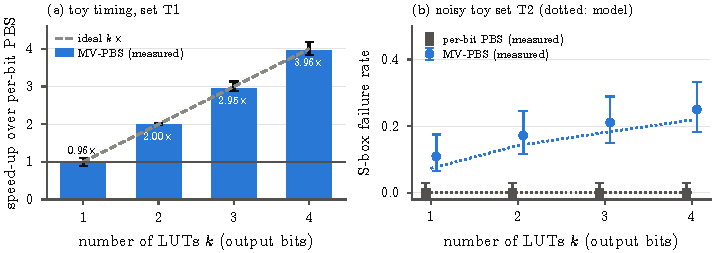
\includegraphics[width=\textwidth]{figs/fig_speedup_failure.pdf}
\caption{(a) Speed-up of \MVPBS{} over per-bit \PBSop{} versus the number of tables $k$ at T1,
bars with paired-bootstrap confidence intervals; dashed: $k\times$. (b) S-box failure rate
(any of the first $k$ bits wrong) at T2 with Wilson intervals; dotted: \Cref{thm:noise}.}
\label{fig:main}
\end{figure}

\noindent\textbf{Noise.} At T1, 0 of 384\evid{E16} evaluated output bits were wrong
(both methods). At T2 the per-bit \PBSop{} output has measured standard deviation
$2^{-8.54}$\evid{E14} (model $2^{-8.50}$\evid{E14}) and never fails (0/128, Wilson upper
end 0.029\evid{E12}), whereas the \MVPBS{} output for bit~0 has $2^{-6.74}$\evid{E13} (model
$2^{-6.84}$\evid{E13}) against a margin of $2^{-6}$\evid{E20}. The S-box failure rate grows with
the number of bits used, from 14/128 at $k=1$ to 32/128 at $k=4$, i.e.\ 0.25
[0.183, 0.332]\evid{E10}; \Cref{thm:noise} with an independence approximation predicts
0.219\evid{E18}. So one blind rotation for all four bits is safe only when the parameters are
chosen for the amplified noise.

\noindent\textbf{A remark on CMux trees.} Vertical packing~\cite{CGGI17} evaluates the whole
table with four CMux gates, but only from GGSW encryptions of the input bits. From a single
LWE ciphertext of the nibble this first requires extracting the bits and circuit-bootstrapping
each of them, which in our toy costs more than one \MVPBS{}; we therefore do not report it as a
competitor.
